\graphicspath{{./images/}}      
\def\CHAPTERONE{./chapters/Chapter-1} 

\chapter{Implementierung}
\label{chap:implementation}
%	\input{\CHAPTERONE /motivation}
\glsresetall
In diesem Kapitel wird beschrieben, wie die implementierten Lösungen vorgestellt. Zuerst wird aufgezeigt, wie die Bildern in der \unreal erstellt wurden. Zur Vereinfachung werden diese  im Folgenden \textit{Unreal-Bilder} genannt. Danach wird die verwendete \gls{ae} erläutert, die die Bilder annotiert und so das Wissen zum  Training eines \gls{mln} extrahiert.

\section{Erstellen der Unreal-Bilder}
\label{sec:takingpics}
Um Unreal-Bilder zum Trainieren eines \gls{mln} zur Verfügung zu haben, müssen diese in der \unreal erstellt werden. Dazu wurde die in Kapitel \ref{subsec:kitchenenvironment} auf Seite \pageref{subsec:kitchenenvironment} vorgestellte Küchenumgebung benutzt. Hier wurden Objekte des täglichen Gebrauchs in der Küche manuell drapiert und mittels des \textit{URoboVision}-Plugins Bilder davon gemacht und an \robosherlock gesendet. Eine solche Anordnung von Objekten in der Küche wird \textit{Szene} genannt. Von jeder Szene wurden Bilder aus mehreren festgelegten Blickwinkeln mittels der \textit{SpawnBox} erstellt. \par 

\textbf{URoboVisionPlugin:} Das Plugin bietet einen in die Szene einfügbaren \textit{ARGBDCameraActor}. Damit wird an \robosherlock ein Farb- und Tiefenbild, sowie ein \textit{ObjectImage} und eine \textit{ObjectMap} gesendet. Auf dem ObjectImage ist jedes Objekt innerhalb der Szene in einer anderen Farbe eingefärbt. Die ObjectMap weist jeder im ObjectImage verwendeten Farbe den Namen des Objektes zu. So kann jedes sichtbare Objekt eindeutig identifiziert werden. Die Bilder habe eine Größe von $1280 \times 960$ Pixeln. \par 

\textbf{Aufnahme aus verschiedene Blickwinkeln:} Die veränderte \textit{SpawnBox} besitzt eine \textit{UBoxComponent}, genannt \textit{SpawnVolume}, aus der vorherigen Iteration. Sie wurde beibehalten, da sie eine visuelle Markierung bietet, wo die Objekte drapiert werden sollten, denn der Mittelpunkt der Box dient als Rotationspunkt, um den ein referenzierter ARGBDCameraActor basierend auf einigen Parametern rotiert wird. Die Kamera wird dabei nach einer bestimmten Zeit in einem einstellbaren Radius $i$-mal um den Mittelpunkt rotiert. Dabei wird die Kamerarotation an der x-Achse der SpawnVolume gespiegelt. Werden zum Beispiel drei Rotationsschritte mit einem Winkel von $30^\circ$ erwünscht, beginnt die Kamera $30^\circ$ links von der x-Achse. Die zweite Position befindet sich dann auf der x-Achse und die dritte Position ist $30^\circ$ rechts von der x-Achse. Der Startpunkt der Kamera auf dem Kreis um die SpawnVolume wird also in Abhängigkeit der Rotationsschritte und des Winkels berechnet. Die Höhe der Kamera kann ebenfalls eingestellt werden, wobei der Mittelpunkt der Box als ebenerdig, also die Höhe 0, angesehen wird. Nach jeder Standortaktualisierung wird die Kamera noch so ausgerichtet, dass sie auf den Mittelpunkt der SpawnVolume schaut. Die Kamera kann auch auf zwei unterschiedlichen Höhen Operieren, wobei der Winkel und die Rotationsschritte unabhängig voneinander eingestellt werden können. \newline
Die einzelnen Parameter und ihre Funktion werden in Tabelle \ref{tab:spawnboxParams} vorgestellt. Der Algorithmus ist in Algorithmus \ref{alg:SpawnBox} beschrieben.

\begin{table}
\rowcolors{1}{}{lightgray}
\begin{tabularx}{\textwidth}{lX}
\textbf{Parameter}  & \textbf{Beschreibung} \\ \hline
SpawnVolume         & Eine Box, die hilft die Objekte zu platzieren. Der Mittelpunkt ist der Rotationspunkt der Kamera.\\  
ScanCamera          & Die Kamera aus dem URoboVision Plugin. \\ 
CameraRadius        & Der Radius des Kreises auf dem die Kamera sich um den Mittelpunkt des SpawnVolume bewegt in UnrealEinheiten.\\ 
CameraHeight        & Die Höhe der Kamera. Der Wert wird auf die Höhe des Mittelpunktes der SpawnVolume addiert in UnrealEinheiten.\\ 
Angle               & Der Winkel, um den die Kamera pro Rotationsschritt rotiert wird in Grad.\\ 
UpdateTime          & Die Zeit die vergeht bis die Kameraposition aktualisiert wird in Sekunden.\\ 
NoOfViewpoints      & Die Anzahl der Blickwinkel, also Rotationsschritte.\\ 
HeightAngle         & Soll eine zweite Höhe benutzt werden, beschreibt dies den Winkel für diese zweite Höhe.\\ 
HeightOffset        & Der Unterschied der zweiten Höhe zur Ersten.\\
NoOfHeightViewpoints & Die Anzahl der Rotationsschritte für die zweite Höhe.\\ 
bUseHeigthViewpoints & Ob die zweite Höhe verwendet werden soll. \\  \hline
\end{tabularx}
\caption{Parameter der \textit{RSpawnbox}}
\label{tab:spawnboxParams}
\end{table}

\begin{algorithm}[H]
\KwData{$Kamera$, $center$ der SpawnBox}
\BlankLine
$processedPoints \gets$ $NoOfViewpoints$ + $NoOfHeightViewpoints$\;
\If{$ProcessedPoints$ == 0}{
	return\;
}
$i \gets$ 0\;
\uIf{$processedPoints$ == $NoOfViewpoints$ + $NoOfHeightViewpoints$}{
	$i \gets$ ComputeVP($CameraRadius$, $CameraHeight$)\;
}\uElseIf{$processedPoints$ == $NoOfHeightViewpoints$}{
	$i \gets$ ComputeVP($CameraRadius$, $CameraHeight$ + $HeightOffset$)\;
}\Else{
	$i \gets$ NextVP($Angle$)\; 
}
$--ProcessedPoints$\;
$Kamera$.SetPosition($i$)\;
$Kamera$.RotateTo($center$)\;
\caption[SpawnBox]{Der Algorithmus der SpawnBox, der die neue Kameraposition berechnet.}
\label{alg:SpawnBox}
\end{algorithm}

Bei der Erstellung der Unreal-Bilder, wurden die Parameter so eingestellt, dass die Kamera auf zwei verschiedenen Höhen Bilder aufnimmt und auf einem Kreis mit dem Radius von 70 Einheiten rotiert. Die Kameraposition wird dabei alle 3 Sekunden aktualisiert, was mit der Aufnahme der RGBD-Kamera synchronisiert wurde. Die erste Höhe ist 35 Einheiten höher als der Mittelpunkt der SpawnVolume. Hier wurden drei Bilder in einem Winkel von $45^\circ$ aufgenommen. Die zweite Höhe ist 35 Einheiten höher als die vorherige. Hier wurden zwei Bilder im Winkel von $45^\circ$ aufgenommen. Eine Szene und ihre fünf Bilder sind in Abbildung \ref{fig:exampleScene} zu sehen. Die Bilder werden an \robosherlock geschickt und hier mittels der \texttt{StorageWriter}-\gls{ae} zur späteren Weiterverarbeitung in einer MongoDB-Instanz gespeichert.

\begin{figure}
\centering
	\begin{subfigure}[b]{0.3\textwidth}
		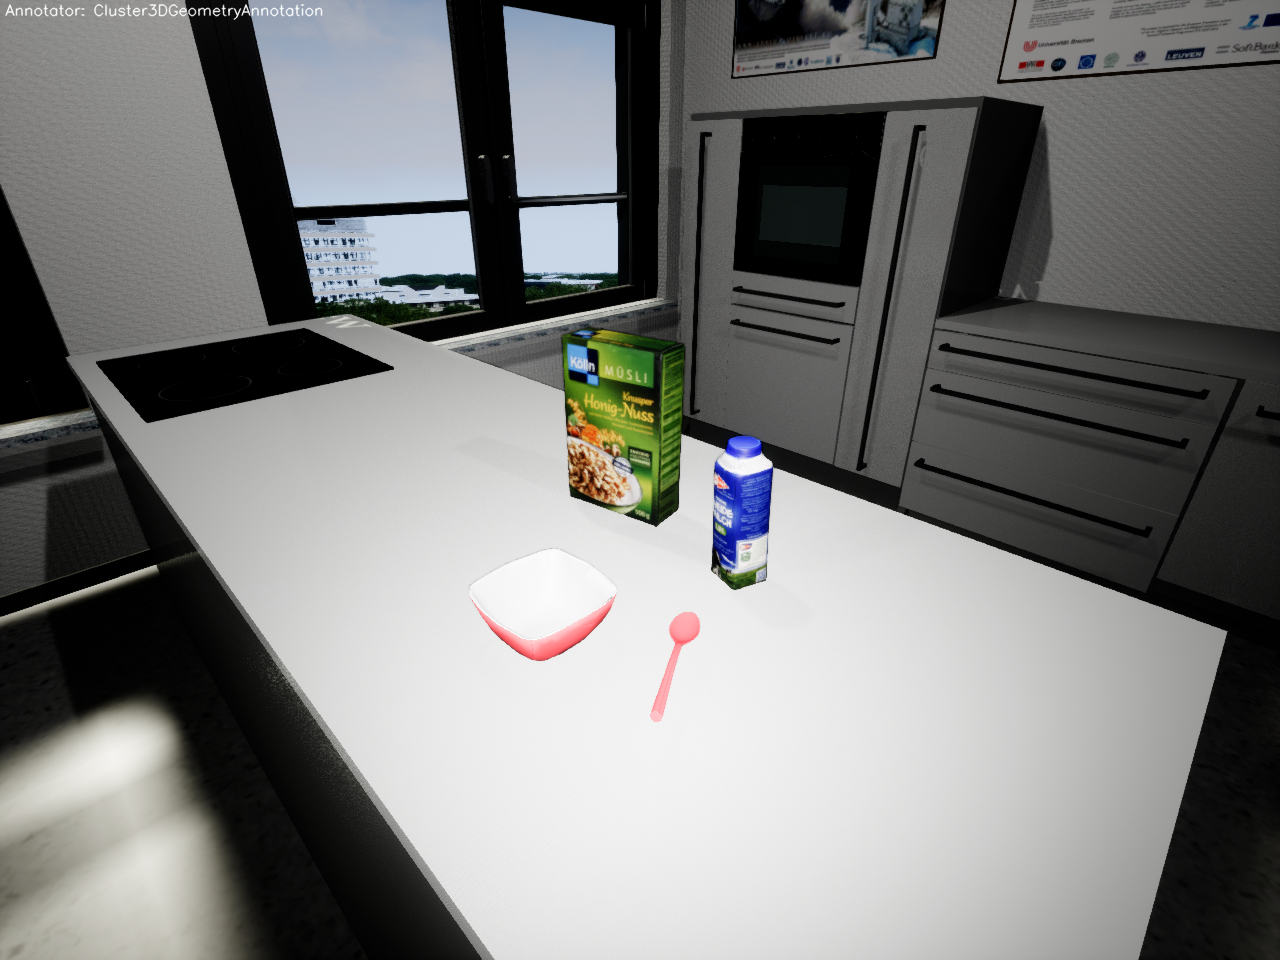
\includegraphics[scale=.1]{img/chapter3/sceneEx_1}
	\end{subfigure}
	\quad
	\begin{subfigure}[b]{0.3\textwidth}
		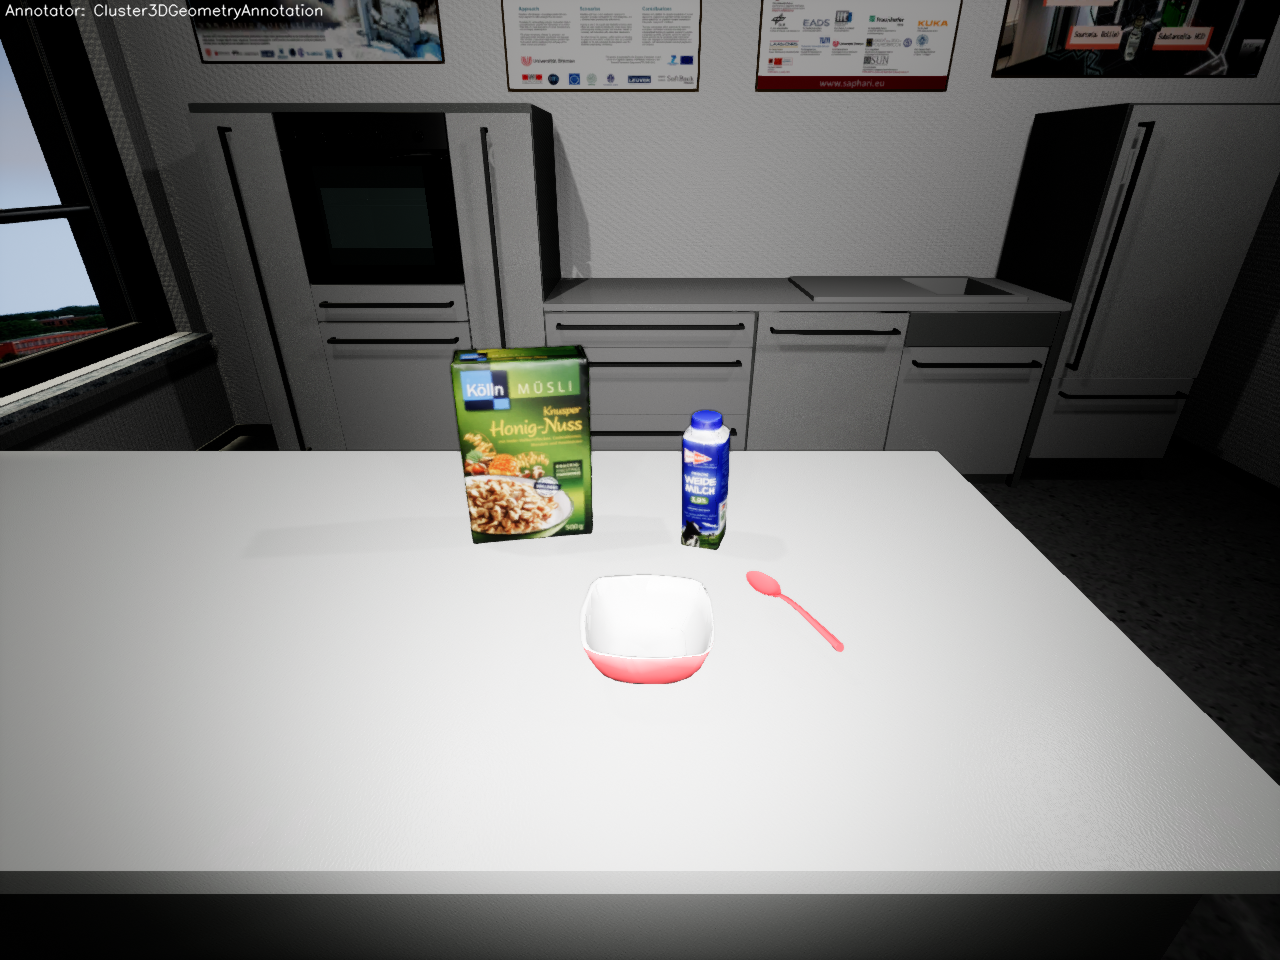
\includegraphics[scale=.1]{img/chapter3/sceneEx_2}	
	\end{subfigure}
	\quad
	\begin{subfigure}[b]{0.3\textwidth}
		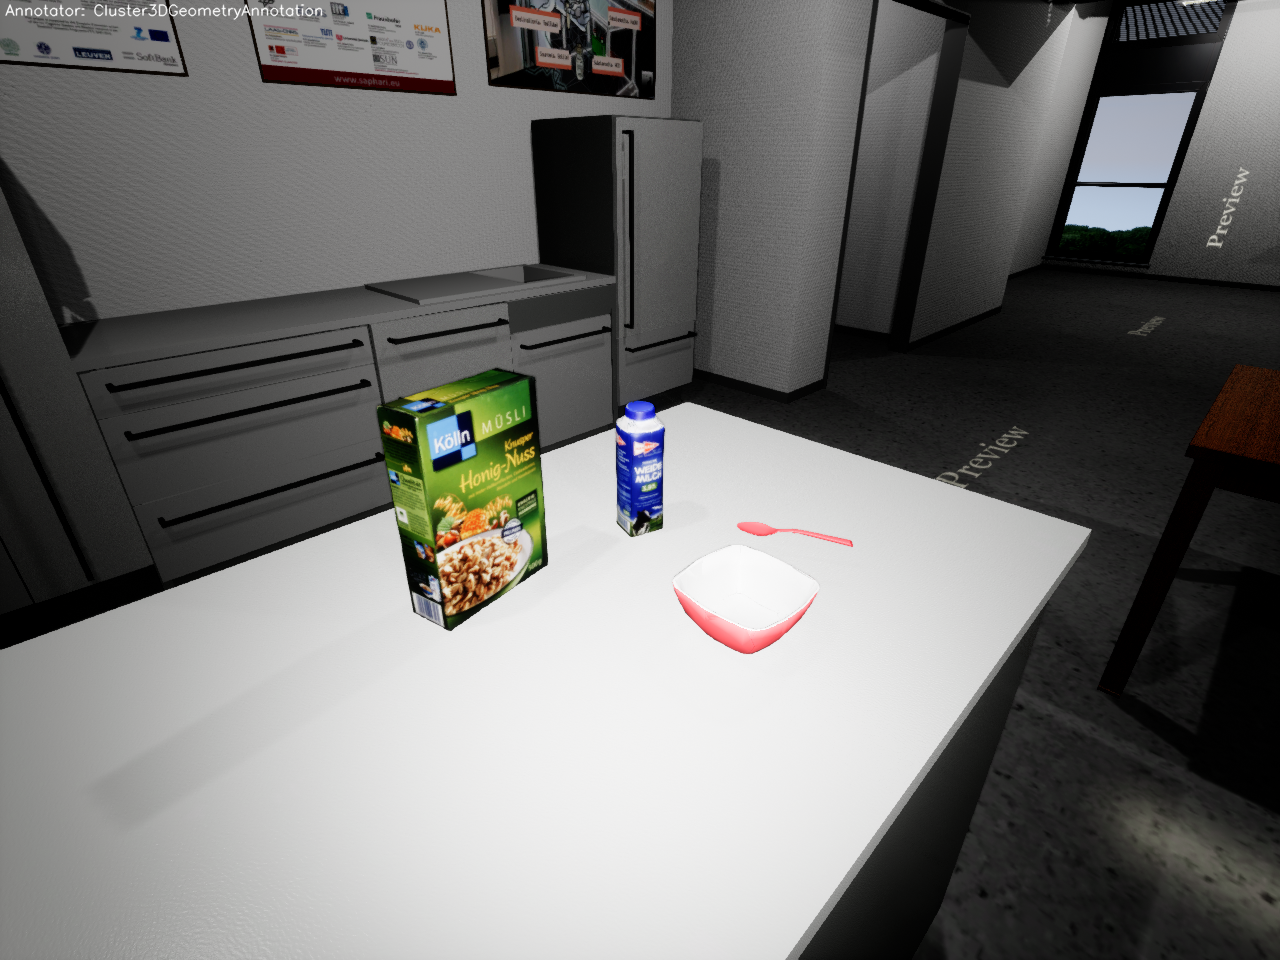
\includegraphics[scale=.1]{img/chapter3/sceneEx_3}	
	\end{subfigure}
	\quad
	\begin{subfigure}[b]{0.3\textwidth}
		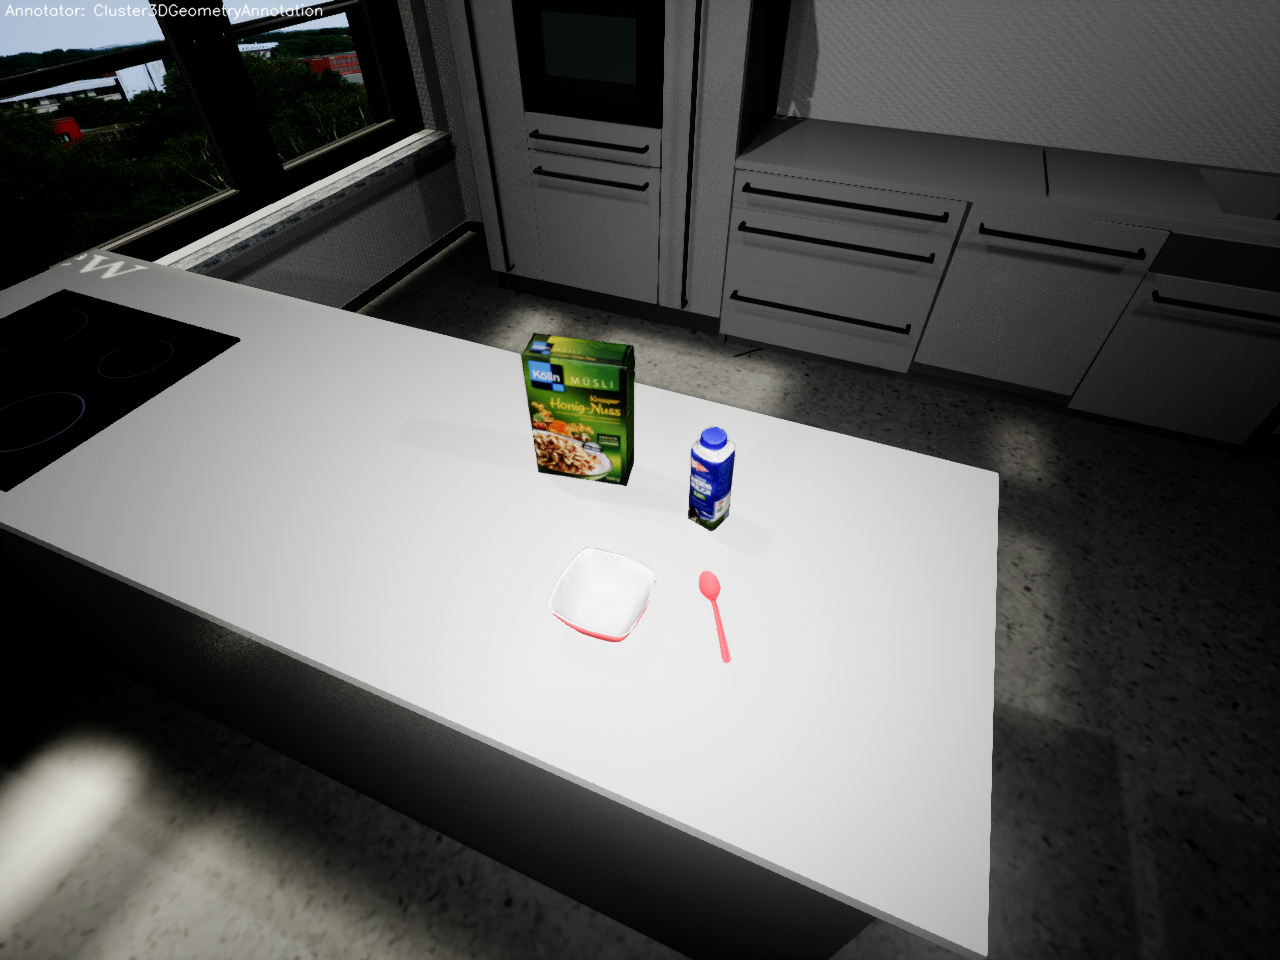
\includegraphics[scale=.1]{img/chapter3/sceneEx_4}	
	\end{subfigure}
	\quad
	\begin{subfigure}[b]{0.3\textwidth}
		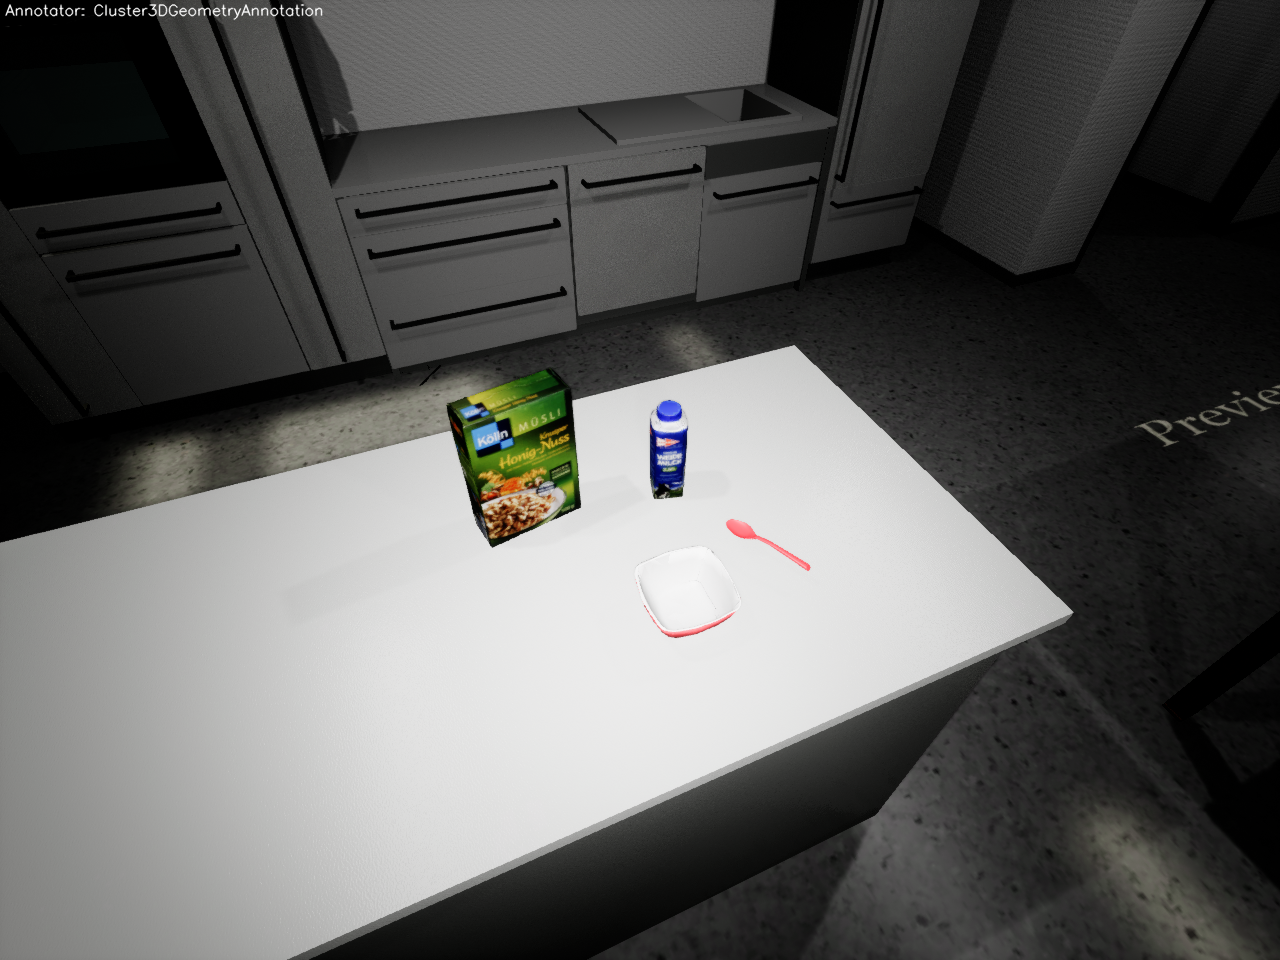
\includegraphics[scale=.1]{img/chapter3/sceneEx_5}	
	\end{subfigure}
\caption[Unreal-Bilder einer Szene]{Die Abbildung zeigt die Bilder der fünf Blickwinkel einer Szene.}
\label{fig:exampleScene}
\end{figure}

\section{Analysis Engine}
\label{sec:analysisengine}
Die Unreal-Bilder können  von einer Perzeptionspipeline in \robosherlock annotiert werden und so die Objektattribute als logische Prädikate zum Training eines \gls{mln} erhalten werden. Dazu werden die Unreal-Bilder aus der Datenbank herausgelesen und als Eingabe verwendet. Auf diesen werden zuerst eine Reihe von \textit{hypotheses generators} zur Segmentierung angewandt mit denen die Objekthypothesen erstellt werden. Dabei werden jedoch auch Objekthypothesen zu Formen und Teilen des Bildes erstellt, die keine für die Arbeit relevanten Objekte, wie die Herdplatte oder dir Front eines Schrankes, sind. Der \texttt{UnrealGTAnnotator} filtert diese \textit{Cluster} nun heraus und annotiert zu den übrig gebliebenen die \gls{gt}. Die noch vorhandenen Hypothesen werden von den Annotatoren auf Eigenschaften analysiert und die Ergebnisse als Annotationen in der \gls{cas} gespeichert. In einem letzten Schritt werden die Annotationen von dem \texttt{MLNInferencer} als logische Prädikate in einer Textdatei ausgeben. \par 

Im Folgenden wird der \texttt{UnrealGTAnnotator} und seine Implementierung erläutert. Danach werden die Annotatoren der Perzeptionspipeline vorgestellt. Tabelle \ref{tab:annotators} bietet eine kurze Übersicht über die Annotatoren, die resultierenden logischen Prädikate und die möglichen Werte.

\subsection{UnrealGTAnnotator}
Der \texttt{UnrealGTAnnotator} filtert alle falschen Objekthypothesen heraus und annotiert für die übrig gebliebenen die \gls{gt}. Dazu wird das \textit{ObjectImage} der Unreal-Bilder verwendet. Der Algorithmus wird im folgenden beschrieben und ist in Algorithmus \ref{alg:UnrealGTAnnotator} in Pseudocode dargestellt. Die einzelnen Teilbilder der RGBD-Kamera pro Unreal-Bild sind deckungsgleich, das heißt die Koordinaten eines Pixels beschreiben in jedem Teilbild den gleichen Punkt. Für jeden Pixel eines Clusters wird nun seine Farbe im ObjectImage betrachtet und so die Anzahl der Pixel, die sich eine Farbe Teilen gezählt. Nun wird für die am meisten vorkommende Farbe in der ObjectMap nachgeschlagen, zu welchem Asset die Farbe gehört. Der Name des Objektes wird mit einer Map verglichen, die den Asset-Namen die \gls{gt} für dieses Objekt zuweist. Wird eine Übereinstimmung des Asset-Namens gefunden, wird für den Cluster die \gls{gt} als \gls{gt}-Annotation zur \gls{cas} hinzugefügt. Die \gls{gt}, die als Annotation hinzugefügt wird, kann vor dem Starten der Pipeline in einer .yaml-Datei, die bei der Initialisierung des Annotators geladen wird, festgelegt werden und ist entweder der Objektname oder der dem Objekt zugewiesene Klassename (für eine Liste der Objektnamen und möglichen \gls{gt} siehe Tabelle \ref{tab:objects} auf S.\pageref{tab:objects}). Wird keine Übereinstimmung gefunden, wird der Cluster verworfen. Es kann allerdings vorkommen, dass eine Objekthypothese korrekt ist, das entsprechende Objekt in seinem ObjectImage jedoch nicht die meisten Pixel belegt. Dies ist vor allem bei Besteck, wie Gabeln und Messern zu beobachten. Um dem vorzubeugen, wird rekursiv auch die zweit- und dritthäufigste Farbe auf eine Übereinstimmung geprüft. Eine Rekursion von drei, hat sich als ausreichend erwiesen, da das Besteck meistens auf einem Tisch liegt, der Cluster also nur aus zwei Farben besteht, und damit schon bei dem zweiten Rekursionsschritt gefunden wird. Auch wenn ein weiteres größeres Objekt mit im Cluster zu finden ist, das nicht zu den relevanten Objekten gehört, wird das Besteck dementsprechend spätestens im dritten Rekursionsschritt gefunden. Weitere Durchläufe sind nicht nötig, da die Objekte so angeordnet wurden, dass es nicht vorkommt, dass drei andere nicht relevante Objekte mehr Pixel innerhalb eines Clusters belegen können, als das relevante Objekt. Es kann allerdings vorkommen, dass ein relevantes Objekt mehr Pixel im Cluster belegt, weshalb die \gls{gt}-Annotationen hinterher manuell überprüft und in den wenigen nötigen Fällen korrigiert wurden.

\begin{algorithm}[H]
\KwData{$objectMap$ = [(ObjectName, Color)], $objectGTMap$ = [(ObjectName, GT)]}
\KwIn{Cluster eines Bildes: $clusters$}
\KwResult{$clusters$ besteht nur aus gewollten Objekthypothesen und deren GT}
\BlankLine
$newClusters$ = []\;
\ForAll{$c \in clusters$}{
	$colorCounter \gets$ map<ObjectName, Occurences>()\;
	\ForAll{Pixels $p \in c$}{
		$color \gets p$.color()\;
		$name \gets objectMap$.getKeyOfValue($color$)\;
		\eIf{$colorCounter$.contains($name$)}{
			$colorCounter$.increaseOccurences($name$)\;
		}{
			$farbZaehler$.insert(pair($name$, 1))\;
		}
	}
	\For{$i \gets 0; i < 3; ++i$}{
		$mostColor \gets$ getNameWithMostOccurences($colorCounter$)\;
		$gt \gets objectGTMap$.find($mostColor$)\;
		\eIf{$gt$.invalid()}{
			$colorCounter$.deleteEntry($mostColor$)\;
		}{
			AnnotateGT($c$, $gt$)\;
			$neueCluster$.add($c$)\;
			break\;
		}
	}	
}
$clusters \gets neueCluster$\;
\caption[UnrealGTAnnotator]{Der Algorithmus des UnrealGTAnnotators filtert die ungewollten Cluster heraus und annotiert für alle anderen die GroundTruth.}
\label{alg:UnrealGTAnnotator}
\end{algorithm}

\subsection{Annotatoren}

Im Folgenden werden die Annotatoren vorgestellt. Sie analysieren die Cluster der Objekthypothesen auf Eigenschaften. Es kommen dabei verschiedene Algorithmen zur Erkennung der Eigenschaften und \glspl{klassifikator} zum Einsatz. Sie sind in einer Perzeptionspipeline zusammengefasst und kommen auch in der Reihenfolge zum Einsatz, in der sie hier vorgestellt werden. Tabelle \ref{tab:annotators} bietet eine kurze Übersicht.

\begin{table}
\rowcolors{1}{}{lightgray}
\begin{tabularx}{\textwidth}{lXX}
\textbf{Annotator}				& \textbf{MLN-Prädikat}	& \textbf{Atome}	\\ \hline 
Cluster3DGeometryAnnotator		& size(cluster, size)	& small, medium, large	\\ 
PrimitiveShapeAnnotator			& shape(cluster, shape)	& box, round, flat 	\\ 
ClusterColorHistogramCalculator  & color(cluster, color)	& red, yellow, green, cyan, blue, magenta, white, black, gray \\ 
GogglesAnnotator				& goggles\_Logo(cluster, logo) \newline googles\_Text(cluster, text)  \newline goggles\_Product(cluster, product)	& 	variabel	\\ 
CaffeAnnotator					& --					& --	\\
PCLFeatureExtractor				& --					& --	\\ 
RfAnnotator						& shape(cluster, shape)	&	box, cylindrical, disk, flat, sphere, other	\\
SVMAnnotator					& instance(cluster, i)	& Instanzname (siehe Tab.\ref{tab:objects}, S.\pageref{tab:objects}) \\
UnrealGTAnnotator				& object(cluster, object)	& Klassen- oder Instanzname (siehe Tab.\ref{tab:objects}, S.\pageref{tab:objects})	\\ \hline 
\end{tabularx}
\caption[Kurzübersicht der Annotatoren]{Eine Kurzübersicht über die Annotatoren und die korrespondieren logischen Prädikate für das \gls{mln}.}
\label{tab:annotators}
\end{table}

\subsubsection{Cluster3DGeometryAnnotator}
Basierend auf der Distanz zwischen Extrempunkten der Objekte, die mit der Entfernung zur Kamera normalisiert wurde, wird dem Objekt eine Größe zugeordnet. Es wird zwischen $big$ und $small$ unterschieden. Das logische Prädikat ist von der Form $size(cluster,  size)$. 

\subsubsection{PrimitiveShapeAnnotator} 
Der \texttt{PrimitiveShapeAnnotator} berechnet die primitive geometrische Form der Objekte.  Dabei wird zwischen $round$ und $box$ unterschieden. Das logische Prädikat ist von der Form $shape(cluster,  shape)$.
   
\subsubsection{ClusterColorHistogramCalculator}
Der \texttt{ClusterColorHistogramCalculator} berechnet für jeden Cluster die Farbverteilung. Daraus bildet er ein Farbhistogramm, das der \gls{cas} hinzugefügt wird. Die unterschiedenen Farben sind: $red$, $yellow$, $green$, $cyan$, $blue$, $magenta$, $white$, $black$ und $gray$. Die am häufigsten auftretende Farbe wird später als logisches Prädikat in der Form $color(cluster,  color)$ ausgegeben. Je nach Häufigkeitsverteilung kann ein Cluster auch zwei Farben haben, die in dem Fall auch beide ausgegeben werden. 

\subsubsection{GogglesAnnotator}
Der \texttt{GooglesAnnotator} benutzt den Webservice \textsc{Google Googles}. Dazu werden die Bilder des Clusters an den Server des Webservices gesendet, der nun Informationen zu den Bildern sucht und zurückgibt. Aus den Ergebnissen werden Logo, Text und Produkt Annotationen erstellt. Die Werte dafür sind abhängig von den Ergebnissen. Da es häufig vorkommt, dass keine Ergebnisse vorliegen, werden in solchen Fällen auch keine Annotationen zur \gls{cas} hinzugefügt. Die logischen Prädikate sind $goggles\_Logo(cluster, logo)$, $googles\_Text(cluster, text)$ und $googles\_Product(cluster, product)$. \par

Theoretisch können die Domänen der Prädikate unendlich groß sein und Störungen unterliegen, da für jeden Cluster ein anderes Atom zustande kommen könnte. Um die Anzahl der Atome zu reduzieren und so jedes Wort durch ein explizit bekanntes Wort zu ersetzen, wird vor dem Training mit den Daten \textit{Clustering} auf die Worte der jeweiligen Prädikate angewandt. Als Algorithmus wurde Affinity-Propagation gewählt und für die Ähnlichkeitsfunktion kommt die Levenshtein-Distanz zum Einsatz. So wird jedes Wort einer Gruppe mit ähnlichen Worten zugeordnet und letztendlich wird jedes Wort durch den zentralen Cluster seiner Gruppe ersetzt. So kommen nur die zentralen Cluster als Atome zum Einsatz.


\subsubsection{CaffeAnnotator}
\label{sec:caffeAnno}
Für den \texttt{CaffeAnnotator} wird das Deep-Learning Framework \textsc{Caffe}\footnote{\url{http://caffe.berkeleyvision.org/}} benötigt. Der Annotator extrahiert Merkmale aus den Bildern und speichert diese als Annotation in der \gls{cas}. Sie werden später für die Klassifikation benötigt.  

\subsubsection{PCLFeatureExtractor}
Wie der \texttt{CaffeAnnotator} fügt der \texttt{PCLFeatureExtractor} Merkmale als Annotationen zur \gls{cas} hinzu. Er extrahiert \gls{vfh}-Merkmale mittels der \gls{pcl} aus den Bildern. Diese werden für den Formklassifikator benötigt.

\subsubsection{RfAnnotator}
Der \texttt{RFAnnotator} klassifiziert die Form der Objekte. Der verwendete \gls{rf} Annotator wurde für die Masterarbeit von Rakibul Islam \cite{rakib} mit einem Objektset der Washington University trainiert. Der \gls{klassifikator} unterscheidet dabei folgende Formen: $box$, $cylindrical$, $disk$, $flat$, $sphere$ und $other$. $shape(cluster, shape)$ ist die Form der logischen Prädikate. Mehr Informationen zu den \glspl{klassifikator} sind in Kapitel \ref{sec:classifiers} auf S. \pageref{sec:classifiers} zu finden.

\subsubsection{SVMAnnotator}
Der \texttt{SVMAnnotator} klassifiziert die Instanz der Objekte. Dazu wurde eine \gls{svm} mit echten Bildern (zu finden im Repository odu\_iai\footnote{\url{https://github.com/bbferka/odu\_iai}}), der in den Experimenten vorkommenden Objekten trainiert. Die Instanz entspricht dabei dem Namen der Objekte und kann in Tabelle \ref{tab:objects} auf S.\pageref{tab:objects} nachgeschlagen werden. Die logischen Prädikate sind von der Form  $instance(cluster, i)$. Mehr Informationen zu \glspl{klassifikator} sind in Kapitel \ref{sec:classifiers} auf S. \pageref{sec:classifiers} zu finden.

\subsubsection{MLNInferencer}
\label{sec:mlnInferencer}
Der \texttt{MLNInferencer} liest die Annotationen aus der \gls{cas} aus und gibt sie als logische Prädikate in einer Textdatei aus. Diese Dateien werden Datenbanken genannt und können als Trainingsdaten für ein \gls{mln} verwendet werden. Der \texttt{MLNInferencer} kann die Prädikate sowohl in \gls{fo} ausgeben, als auch in \textit{Fuzzy-Logik}. Dabei werden für jedes Prädikat die Konfidenzen der Annotatoren mit ausgegeben. Zusätzlich wird noch ein manuell festgesetztes scene-Prädikat ausgegeben, dass näher in Kapitel \ref{chap:experiments} beschrieben wird. Abbildung \ref{inferencerExample} zeigt die Ausgabe für ein Bild mit 3 Objekten. 

\begin{figure}
\begin{lstlisting}[backgroundcolor=\color{backcolour}]
scene(cooking)

shape(c0,round)
size(c0,large)
color(c0,red)
color(c0,yellow)
shape(c0,cylindrical)
instance(c0,MondaminPancakeMix)
object(c0,TomatoSauce)

shape(c1,box)
shape(c1,flat)
size(c1,small)
color(c1,white)
shape(c1,box)
instance(c1,MondaminPancakeMix)
object(c1,PancakeMix)

shape(c2,box)
size(c2,small)
color(c2,white)
color(c2,blue)
shape(c2,box)
instance(c2,SpitzenReis)
object(c2,Rice)
\end{lstlisting}  
\caption[Beispiel für die Ausgabe des MLNInferencer]{Beispiel für die Ausgabe der logischen Prädikate des MLNInferencer für ein Bild.}
\label{inferencerExample}
\end{figure}

\begin{table}
\rowcolors{1}{}{lightgray}
\begin{tabularx}{\textwidth}{llccccc}
\textbf{Instanz}  				& \textbf{Klasse}	& \textbf{breakfast}	& \textbf{fridge}	& \textbf{cooking}	& \textbf{Unreal} & \textbf{Real} \\ \hline
AlbiHimbeerJuice				& Juice				& +			& +			& +			& 14	& 18	\\
BlueCeramicIkeaMug				& DrinkingMug		& +			& 			&			& 8		& 9\\
BlueMetalPlateWhiteSpeckles		& DinnerPlate		& 			& 			&	+		& 9		& 10\\
BluePlasticBowl					& Bowl				& +			& 			&			& 9		& 9\\
BluePlasticFork					& Fork				& 			& 			&	+		& 8		& 9\\
BluePlasticKnife				& Knife				& 			& 			&	+		& 8		& 9\\
BluePlasticSpoon				& Spoon				& +			& 			&			& 8		& 11\\
CupEcoOrange					& Cup				& +			& 			&	+		& 12	& 15\\
EdekaRedBowl					& Bowl				& +			& 			&			& 8		& 9\\
ElBrygCoffee					& Coffee			& +			& 			&			& 8		& 9\\
JaMilch							& Milk				& +			& +			&			& 13	& 14\\
JodSalz							& TableSalt			& 			& 			&	+		& 9		& 9\\
KelloggsCornFlakes				& BreakfastCereal	& +			& 			&			& 8		& 9\\
KelloggsToppasMini				& BreakfastCereal	& +			& 			&			& 8		& 9\\
KnusperSchokoKeks				& BreakfastCereal	& +			& 			&			& 8		& 8\\
KoellnMuesliKnusperHonigNuss	& BreakfastCereal	& +			& 			&			& 8		& 8	\\
LargeGreySpoon					& Spoon				& 			& 			&	+		& 9		& 8	\\
LinuxCup						& DrinkingMugin		& +			& 			&			& 8		& 0\\
LionCerealBox					& BreakfastCereal	& +			& 			&			& 8		& 9	\\
MarkenSalz						& TableSalt			& 			& 			&	+		& 9		& 8	\\
MeerSalz						& TableSalt			& 			& 			&	+		& 9		& 8	\\
MondaminPancakeMix				& PancakeMix		& 			& 			&	+		& 9		& 8	\\
NesquikCereal					& BreakfastCereal	& +			& 			&			& 8		& 9	\\
PfannerGruneIcetea				& Tea-Iced			& 			& +			&	+		& 13	& 14\\
PfannerPfirsichIcetea			& Tea-Iced			& 			& +			&	+		& 14	& 13\\
RedMetalBowlWhiteSpeckles		& Bowl				& +			& 			&			& 9		& 8\\
RedMetalCupWhiteSpeckles		& Cup				& +			& 			&			& 8		& 10\\
RedMetalPlateWhiteSpeckles		& DinnerPlate		& 			& 			&	+		& 9		& 9\\
RedPlasticFork					& Fork				& 			& 			&	+		& 8		& 9\\
RedPlasticKnife					& Knife				& 			& 			&	+		& 8		& 9\\
RedPlasticSpoon					& Spoon				& +			& 			&			& 9		& 10\\
ReineButterMilch				& Buttermilk		& +			& +			&			& 13	& 14\\
SeverinPancakeMaker				& PancakeMaker		& 			& 			&	+		& 10	& 10\\
SiggBottle						& DrinkingBottle	& 			& 			&	+		& 9		& 9\\
SlottedSpatula					& Spatula			& 			& 			&	+		& 9		& 8\\
SojaMilch						& Milk				& +			& +			&			& 13	& 14\\
SpitzenReis						& Rice				& 			& 			&	+		& 9		& 9\\
TomatoAlGustoBasilikum			& TomatoSauce		& 			& 			&	+		& 8		& 8\\
TomatoSauceOroDiParma			& TomatoSauce		& 			& 			&	+		& 9		& 8\\
VollMilch						& Milk				& +			& +			&			& 13	& 14\\
WeideMilchSmall					& Milk				& +			& +			&			& 13	& 14\\
WhiteCeramicIkeaBowl			& Bowl				& +			& 			&			& 8		& 9\\
YellowCeramicPlate				& DinnerPlate 	    & 			& 			&	+		& 9		& 6\\ \hline
\textbf{Insgesamt: 43}				& \textbf{20}		& \textbf{23} & \textbf{8} & \textbf{22} & & \\
\end{tabularx}
\caption[Objekte und ihre Verteilung in den Szenen]{Die Tabelle enthält alle Objekte und welchen Klassen sie zugeordnet sind, sowie die Zuordnung zu den Szenarien und wie häufig sie insgesamt in den Szenen vorkommen.}
\label{tab:objects}
\end{table}
